\setcounter{page}{1}
\section{Theorie}
\label{sec:theorie}
Es wird die Ausbreitung der magnetischen Flussdichte
\begin{equation}
  \vec{B} = μ \cdot \vec{H}
  \label{eqn:erste}
\end{equation}
in Abhängigkeit zur Permeabilität $μ$ und der Feldstärke $\vec{H}$ untersucht.
Innerhalb eines Vakuums existiert die Vakuum-Permeabilität $μ_0$.
Im Gegensatz dazu wird die materialabhängige Permeabilität als relative Permeabilität $μ_r$ bezeichnet.
Es wird vorausgesetzt, dass die Medien homogen sind, damit die Induktionskonstante verlässlich ist.
Der Leiter eines elektrischen Stromdurchflusses ist von einem Magnetfeld umgeben dessen Feldlinien konzentrische Kreise beschreiben.
Der Stromfluss innerhalb dieses Leiters verläuft in einer senkrechten Achse zu den Kreisen.
Der Abstand des Magnetfeldes weist eine Magnetfeldstärke $\vec{H}$ auf, die in
Beziehung zu dem Stromdurchflusses des Leiters steht.
Das Biot-Savartsche Gesetz \cite{Anleitung}
\begin{equation}
  \symup{d}\vec{B}=\frac{μ_0 \cdot I}{4 π}\frac{\symup{d}\vec{s}\times \vec{r}}{r^3}
\end{equation}
stellt diesen Zusammenhand her.
Die Vakuum-Permeabilität $μ_0$ wird mit der Konstante $μ_0 = 4 π \cdot 10^{-7} \:\si{\newton\per\ampere\squared}$ bezeichnet.
I beschreibt den Strom, der durch den Leiter fließt.
Das Magnetfeld einer Strom führenden Windung der Spule kann mit diesem Gesetz berechnet werden.

\subsection{Magnetfeld eines stromdurchflossenen langestreckten Leiters}

Die Flussdichte eines einfachen langestreckten Leiters wird ermittelt durch
\begin{align}
  \vec{B}(x)=\frac{μ_0 I}{2}\frac{R^2}{(R^2+x^2)^{3/2}}\cdot x \:.
\end{align}

\begin{figure}
  \centering
  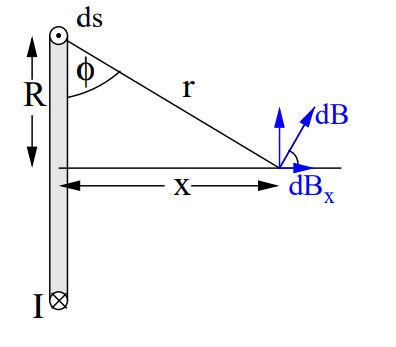
\includegraphics[width=11cm, height=8cm]{content/bilder/Spule1.PNG}
  \caption{Skizze zur Berechnung des Magnetfeldes eines stromdurchflossenen langestreckten Leiter (Solenoid).\cite{Anleitung}}
  \label{fig:Spule1}
\end{figure}

\noindent Der magnetische Fluss erhöht sich in Abhängigkeit der Windungsanzahl.
Die magnetische Feldstärke ist in der Mitte des Solenoiden konstant.
Innerhalb der Spule treten Feldlinien auf, die parallel zur Achse verlaufen.
In diesem Bereich wird das magnetische Feld als homogen bezeichnet.
Im Gegensatz dazu fächern sich die Feldlinien außerhalb der Spulen auf,
sodass der magnetische Fluss in diesem Bereich als inhomogen bezeichnet wird.
Das entstehende homogene Feld $B$ ist dabei proportional zur Spulenlänge $L$,
sowie der Windungszahl $N$ und dem Spulenstrom $I$. $B$ berechnet sich aus
\begin{equation}
  B = μ_0 μ_r \frac{N}{L}I \:.
\end{equation}
In der Abbildung \ref{fig:Spule1} wird der Aufbau des Magnetfeldes eines langestreckten,
stabförmigen, stromdurchflussenen, Leiters dargestellt.
Die Ausrichtung des Magnetfeldes wird dabei mit den Vektoren charakterisiert.
Für eine Spule mit $n$ Windungen folgt
\begin{equation}
      B(x) = \frac{μ_0 n I}{2} \left(\frac{x+L}{\sqrt{(x+L)^2 + R^2}} - \frac{x}{\sqrt{x^2 + R^2}} \right) \:.
      \label{eqn:theoriespule}
\end{equation}
\subsection{Magnetfeld eines stromdurchflossenen Kreisringes}
Wenn der Solenoid zu einem Ring (Torus) gebogen ist, existieren keine Randeffekte.
Außerhalb des Torus ist deshalb das Magnetfeld gleich Null.
Innerhalb des Torus ist das Magnetfeld homogen, sodass $L=2 π r_T$ wird.
$B$ wird wie folgt berechnet
\begin{equation}
  B = μ_0 μ_r \frac{N}{2 π r_T}I \:.
\end{equation}

\subsection{Magnetfeld einer Helmholtz-Spule}
Eine Helmholtz-Spule besteht aus zwei gleichartigen koaxialen Kreisringen,
mit dem Radius $R$ und dem Abstand $R$ voneinander. Bei diesem Spulenaufbau entsteht ein homogenes Magnetfeld.
Beide Spulen werden dabei gleichsinnig vom Strom $I$ durchflossen.

\begin{figure}
  \centering
  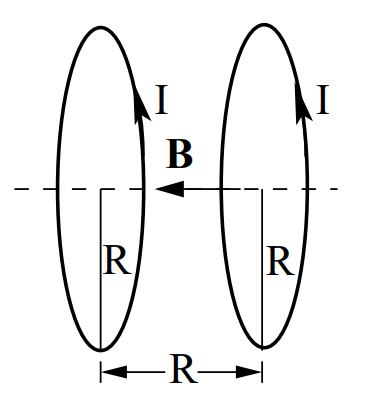
\includegraphics[width=11cm, height=8cm]{content/bilder/Spule2.PNG}
  \caption{Das Helmholtzspulenpaar.\cite{Anleitung}}
  \label{fig:Spule2}
\end{figure}

\noindent Die Achsen der beiden Spulen fallen zusammen.
Das Magnetfeld $B$ ist innerhalb der Spulen homogen.
Es wird ebenfalls mit dem Biot-Savartschen Gesetz berechnet.
Durch Überlagerung der Magnetfelder der einzelnen Spulen entsteht der Ursprung des Feldes in der Mitte des Spulenabstandes.
Dies gilt aber nur wenn der Spulenabstand $R$ gleich dem Radius der Einzelspule $R$ ist.
Dieser Sachverhalt wird in Abbildung \ref{fig:Spule2} skizziert.
Sind Abstand und Spulenradius nicht identisch, so wird das Feld in der Mitte der Helmholtz-Spule wie folgt berechnet
\begin{equation}
  B(0) = \frac{μ I R^2}{(R^2+x^2)^{3/2}} \:.
  \label{eqn:helmtheorie}
\end{equation}
$B_0$ definiert den Mittelpunkt des Abstandes beider Spulen.
$x$ bezeichnet dabei den jeweiligen Abstand zum Mittelpunkt.

\subsection{Magnetfelder ferromagnetischer Materialien}

Ferromagnetische Stoffe, wie zum Beispiel Eisen, unterscheiden sich von anderen Materialien,
weil sie ein permanentes, magnetisches Moment besitzen, das heißt sie sind ohne äußeren Einfluss magnetisch.
Die magnetischen Momente richten sich innerhalb einzelner Bereiche (Weiß´sche Bezirke) parallel zueinander aus.
Die Richtungsänderung der magnetischen Momente erfolgt durch ein äußeres Magnetfeld,
sodass eine Vergrößerung der Weiß´schen Berzirke erfolgen kann.
Es kann eine vollständige Übereinstimmung in der Aussrichtung der magnetischen Momente und der äußeren Magnetfeldes erreicht werden.
Die Flussdichte in ferromagnetischen Materialien ist sehr hoch und so wird sie nicht über Formel \ref{eqn:erste} berechnet.
Sie wird in der Hysteresekurve (Magnetisierungskurve) dargestellt.

\begin{figure}
  \centering
  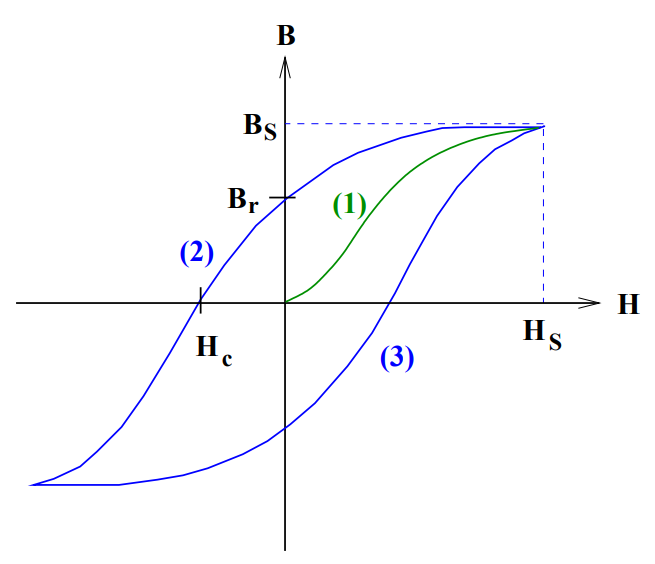
\includegraphics[width=11cm, height=8cm]{content/bilder/Spule3.PNG}
  \caption{Schematischer Verlauf der Hysteresekurve.\cite{Anleitung}}
  \label{fig:Spule3}
\end{figure}

Die Darstellung der Kurve ist nicht stärker definierbar, weil sie von dem zu untersuchenden Material abhängt.
Innerhalb einer nicht magnetisierten Probe sind die magnetischen Momente statistisch so verteilt, dass sich $B(H=0)=0$ ergibt.\\
Durch äußere Magnetfelder erhöht sich die Magnetisierung der Probe bis sie den Sättigungswert $B_s$ erreicht.
Wird das äußere Magnetfeld verringert bilden sich Bereiche mit entgegengesetzter Magnetisierung aus
(Kurve 2 in Abbildung \ref{fig:Spule3}). Ohne Fortbestand des Magnetfeldes bleibt
eine Remanenz $B_r(H=0)\neq 0$. Eine Aufhebung dieser Remanenz ist möglich,
wenn ein magnetisches Gegenfeld (Koerzitivkraft) $H_c$ erzeugt wird.
Der Magnetismus wird negativ und zeigt in die Richtung des Gegenfeldes bis der Sättigungswert $-B_s$ erreicht wird.
Bei Erhöhung des äußeren Magnetfeldes (Kurve 3) entsteht die Hysteresekurve,
eine zum Ursprung punktsymmetrische Kurve. Bei ferromagnetischen Materialien stellt sich die Permeabilität
$μ_r$ also als Funktion der magnetischen Feldstärke $H$ dar.
Die differentielle Permeabilität $μ_{\text{diff}}$ ergibt sich deshalb aus
\begin{equation}
  μ_{\text{diff}} = \frac{1}{μ_0}\frac{\symup{d}B}{\symup{d}H} \:.
\end{equation}
Spulen mit ferromagnetischer Füllung verfügen über einen erhöhten magnetischen Fluss der Spule.
Hierbei ist ebenfalls die Abhängigkeit von der Magnetisierung M zu sehen.
Für die Feldstärke gilt $\vec{B_{Fe}} =μ \vec{M}$
Der unmagnetische Fluss der Spule mit Eisenkern ermittelt sich über
\begin{equation}
  \vec{B} = μ_0 (\vec{H}+\vec{M}) \:.
\end{equation}
Wird ein Torus als Spule benutzt treten keine Randeffekte auf und es gilt
$\vec{H}=\vec{H_0}=\sfrac{\vec{B}}{μ_0}$, weil die relative Permeabilität in einer
Größenordnung von $10^2$ bis $10^7$ liegt, reduziert sich die Gleichung zu $\vec{B}\approx μ \vec{M}$.
